\documentclass[10pt,a4paper]{article}
\usepackage[a4paper,margin=2cm]{geometry}
\usepackage[utf8]{inputenc}
\usepackage[T1]{fontenc}
\usepackage{amsmath,amssymb}
\usepackage{mathptmx}
\usepackage{graphicx,booktabs,array,xcolor,caption,float,enumitem}
\usepackage[hidelinks]{hyperref}
\captionsetup{font=small,labelfont=bf}
\captionsetup[figure]{labelformat=empty}
\setcounter{secnumdepth}{0}
\setlength{\parskip}{3pt}
\setlength{\parindent}{0pt}
\setlist{nosep,leftmargin=1.2em}
\renewcommand{\figurename}{Gambar}
\renewcommand{\tablename}{Tabel}
\newcommand{\KELAS}{[isi kelas]}
\newcommand{\GITHUB}{https://github.com/[username]/[nama-repo]}
\newcommand{\MLPacc}{88{,}93}
\newcommand{\WoneOrth}{17{,}6}
\newcommand{\WoneCond}{39{,}0}
\newcommand{\WoneSVmax}{14{,}0}
\newcommand{\ReluOne}{74{,}1\%}
\newcommand{\ReluTwo}{51{,}5\%}
\newcommand{\ZeroFrac}{51{,}5\%}
\newcommand{\NegFrac}{19{,}7\%}
\newcommand{\TtwoMSE}{0{,}1136}
\newcommand{\TtwoPSNR}{9{,}57}
\newcommand{\TtwoSSIM}{0{,}122}
\newcommand{\TthreeMSE}{0{,}3065}
\newcommand{\TthreePSNR}{5{,}19}
\newcommand{\TthreeSSIM}{0{,}066}
\newcommand{\TpinvMSE}{0{,}1871}
\newcommand{\TpinvPSNR}{7{,}94}
\newcommand{\TpinvSSIM}{0{,}014}
\newcommand{\FdMSE}{0{,}0176}
\newcommand{\FdPSNR}{18{,}31}
\newcommand{\FdSSIM}{0{,}658}
\newcommand{\FdVar}{0{,}671}
\newcommand{\FdAcc}{87{,}9}
\newcommand{\AeMSE}{0{,}0065}
\newcommand{\AePSNR}{22{,}98}
\newcommand{\AeSSIM}{0{,}829}
\newcommand{\AeVar}{0{,}864}
\newcommand{\AeAcc}{87{,}6}
\newcommand{\FdAeRatio}{2{,}7}
\newcommand{\NNrand}{17{,}72}
\newcommand{\NNreal}{3{,}44}
\newcommand{\NNratio}{5{,}2}
\newcommand{\EntMLP}{0{,}617}
\newcommand{\EntVAE}{0{,}473}
\newcommand{\EntReal}{0{,}176}
\newcommand{\TrouserMLP}{57}
\newcommand{\FIDmlp}{149{,}1}
\newcommand{\FIDvae}{89{,}2}
\newcommand{\TAE}{2{,}7}
\newcommand{\LAE}{0{,}37}
\newcommand{\PAE}{0{,}44}
\newcommand{\MSEAE}{0{,}0065}
\newcommand{\PSNRAE}{22{,}98}
\newcommand{\SSIMAE}{0{,}829}
\newcommand{\TSAE}{3{,}0}
\newcommand{\LSAE}{0{,}36}
\newcommand{\PSAE}{0{,}44}
\newcommand{\MSESAE}{0{,}0097}
\newcommand{\PSNRSAE}{21{,}12}
\newcommand{\SSIMSAE}{0{,}762}
\newcommand{\TVAE}{4{,}0}
\newcommand{\LVAE}{0{,}18}
\newcommand{\PVAE}{0{,}45}
\newcommand{\MSEVAE}{0{,}0132}
\newcommand{\PSNRVAE}{19{,}64}
\newcommand{\SSIMVAE}{0{,}708}
\newcommand{\FIDVAE}{89{,}2}
\newcommand{\COVVAE}{0{,}990}
\newcommand{\MINCVAE}{138}
\newcommand{\MAXCVAE}{292}
\newcommand{\TGAN}{14{,}6}
\newcommand{\LGAN}{1{,}20}
\newcommand{\PGAN}{1{,}49}
\newcommand{\FIDGAN}{124{,}6}
\newcommand{\COVGAN}{0{,}991}
\newcommand{\MINCGAN}{113}
\newcommand{\MAXCGAN}{267}
\newcommand{\TDCGAN}{182{,}0}
\newcommand{\LDCGAN}{22{,}19}
\newcommand{\PDCGAN}{1{,}78}
\newcommand{\FIDDCGAN}{31{,}9}
\newcommand{\COVDCGAN}{0{,}998}
\newcommand{\MINCDCGAN}{171}
\newcommand{\MAXCDCGAN}{230}
\newcommand{\TDDPM}{478{,}5}
\newcommand{\LDDPM}{93821}
\newcommand{\PDDPM}{1{,}25}
\newcommand{\FIDDDPM}{28{,}0}
\newcommand{\COVDDPM}{0{,}992}
\newcommand{\MINCDDPM}{127}
\newcommand{\MAXCDDPM}{267}
\newcommand{\LDDPMstep}{92{,}4}
\newcommand{\LVAErec}{0{,}37}
\newcommand{\FIDreal}{8{,}4}
\newcommand{\FIDaegauss}{206{,}7}
\newcommand{\FIDsaegauss}{152{,}4}
\newcommand{\COVAEgauss}{0{,}932}
\newcommand{\COVSAEgauss}{0{,}956}
\newcommand{\COVmlp}{0{,}929}
\newcommand{\COVreal}{0{,}998}
\newcommand{\DDPMxGAN}{4227}
\newcommand{\ZFAE}{0{,}0\%}
\newcommand{\ACTAE}{64{,}0}
\newcommand{\DEADAE}{0}
\newcommand{\ZFSAE}{55{,}8\%}
\newcommand{\ACTSAE}{28{,}3}
\newcommand{\DEADSAE}{33}
\newcommand{\VOIDAE}{1{,}58}
\newcommand{\VOIDENDAE}{1{,}17}
\newcommand{\VOIDSAE}{2{,}00}
\newcommand{\VOIDENDSAE}{1{,}49}
\newcommand{\VOIDVAE}{1{,}45}
\newcommand{\VOIDENDVAE}{1{,}15}
\newcommand{\ENTMIDAE}{1{,}45}
\newcommand{\STEPAE}{0{,}0268}
\newcommand{\ENTMIDSAE}{0{,}90}
\newcommand{\STEPSAE}{0{,}0266}
\newcommand{\ENTMIDVAE}{1{,}33}
\newcommand{\STEPVAE}{0{,}0449}
\newcommand{\ENTMIDGAN}{0{,}05}
\newcommand{\STEPGAN}{0{,}1142}
\newcommand{\ENTMIDDCGAN}{0{,}25}
\newcommand{\STEPDCGAN}{0{,}0865}
\newcommand{\DRGAN}{0{,}533}
\newcommand{\DFGAN}{0{,}468}
\newcommand{\GNGANfirst}{4{,}01}
\newcommand{\GNGANlast}{1{,}07}
\newcommand{\GSTDGAN}{0{,}075}
\newcommand{\DRDCGAN}{0{,}552}
\newcommand{\DFDCGAN}{0{,}448}
\newcommand{\GNDCGANfirst}{4{,}80}
\newcommand{\GNDCGANlast}{2{,}06}
\newcommand{\GSTDDCGAN}{0{,}201}
\newcommand{\AEtrain}{0{,}0063}
\newcommand{\AEval}{0{,}0066}
\newcommand{\BoneVAE}{0{,}04}
\newcommand{\BoneGAN}{0{,}21}
\newcommand{\BoneDCGAN}{1{,}60}
\newcommand{\AUCAE}{0{,}762}
\newcommand{\ERRNAE}{0{,}0065}
\newcommand{\ERRDAE}{0{,}0115}
\newcommand{\FIXAE}{0{,}154}
\newcommand{\AUCSAE}{0{,}742}
\newcommand{\ERRNSAE}{0{,}0097}
\newcommand{\ERRDSAE}{0{,}0159}
\newcommand{\FIXSAE}{0{,}202}
\newcommand{\PSNRdropSAE}{1{,}9}
\newcommand{\KLVAE}{15{,}9}
\newcommand{\GANoverDCGAN}{3{,}9}
\newcommand{\DDPMfirst}{0{,}1116}
\newcommand{\DDPMlast}{0{,}0414}
\newcommand{\DDPMval}{0{,}0402}
\newcommand{\QoneFID}{FID dari prior $\mathcal{N}(0,I)$ (makin kecil makin baik) berurutan: DDPM (28{,}0) $<$ DCGAN (31{,}9) $<$ VAE (89{,}2) $<$ Vanilla GAN (124{,}6); sebagai batas bawah, FID antara dua himpunan citra riil adalah 8{,}4.}
\newcommand{\FigTwoText}{Sampel VAE (A) memiliki siluet benar dan beragam tetapi buram serta kontrasnya rendah: decoder mengeluarkan $\mathbb{E}[x|z]$ sehingga tekstur kain hilang. Vanilla GAN (B) menghasilkan siluet tajam dan berkontras tinggi, tetapi setiap piksel berbintik seperti derau garam-merica, karena generator FC tidak memiliki bias korelasi spasial antarpiksel; inilah sebabnya FID-nya (124{,}6) bahkan lebih buruk daripada VAE (89{,}2). DCGAN (C) menghasilkan kontur bersih, permukaan halus, dan detail seperti tali tas serta sol sepatu. DDPM (D) menghasilkan sampel dengan tekstur dan detail lokal paling alami serta FID terbaik (28{,}0). Dari sisi keragaman, keempat model menutup 10 kelas hampir merata (coverage 0{,}990--0{,}998), sehingga tidak ada mode collapse tingkat kelas.}
\newcommand{\TrilemmaText}{Generative trilemma (Xiao dkk., 2022) menyatakan bahwa sulit mendapatkan sekaligus kualitas sampel tinggi, sampling cepat, dan mode coverage. Hasil kami mengonfirmasinya. VAE: cepat (0{,}18 ms/64) dan coverage tinggi, tetapi kualitas rendah (FID 89{,}2). DCGAN: cepat (22{,}19 ms/64) dan berkualitas (FID 31{,}9); coverage tingkat kelas baik, tetapi secara teoretis rentan mode dropping karena divergensi mode-seeking dan tidak memiliki likelihood untuk memverifikasinya. DDPM: coverage dijamin oleh objektif likelihood-bound dan FID 28{,}0, tetapi sampling 1000 langkah butuh 93{,}8 detik per batch 64, yaitu 4227$\times$ lebih lambat daripada DCGAN. Latensi DDPM berbanding lurus dengan jumlah langkah $T$; inilah harga dari kestabilan dan coverage.}
\newcommand{\AvatarText}{Latensi per citra (batch 1, CPU 2 thread) adalah VAE 0{,}04 ms, Vanilla GAN 0{,}21 ms, dan DCGAN 1{,}60 ms; untuk batch 64 masing-masing 0{,}18, 1{,}20, dan 22{,}19 ms. Ketiganya jauh di bawah anggaran 30 ms karena sama-sama single-pass, sedangkan DDPM (sekitar 1466 ms per citra) mustahil dipakai. Di antara kandidat yang memenuhi latensi, DCGAN memberi kualitas terbaik (FID 31{,}9 vs VAE 89{,}2 dan Vanilla GAN 124{,}6). Konvolusi juga lebih ramah akselerator mobile (NPU/GPU) dan parameternya dapat dikuantisasi. Vanilla GAN tidak direkomendasikan karena artefak bintiknya sangat terlihat pada wajah/avatar. VAE cocok bila yang dibutuhkan adalah kontrol laten yang halus (misalnya slider atribut), dengan konsekuensi hasil lebih buram. Untuk produk nyata, generator DCGAN perlu dikondisikan pada citra input (image-to-image).}
\newcommand{\CreativeChoice}{DDPM}
\newcommand{\CreativeText}{DDPM memberi FID terbaik (28{,}0 vs DCGAN 31{,}9) walaupun hanya dilatih 12 epoch di CPU, dengan loss yang turun monoton tanpa tuning keseimbangan $G$/$D$. Untuk aset beresolusi dan berfidelitas tinggi, faktor penentunya adalah inductive bias dan skalabilitas. DDPM memecah generasi menjadi ratusan langkah denoising kecil yang masing-masing merupakan regresi stabil, sehingga mudah diskalakan ke resolusi dan kapasitas besar, menutup seluruh mode data, serta mendukung conditioning (teks, inpainting, guidance). DCGAN pada resolusi tinggi terkenal sulit distabilkan dan rentan mode dropping. Latensi sampling yang tinggi tidak kritis dalam pipeline kreatif offline, dan dapat dipangkas dengan sampler yang lebih sedikit langkahnya (misalnya DDIM).}
\newcommand{\ABSTRAK}{Pada rekonstruksi, Vanilla AE unggul (PSNR 22{,}98 dB) atas Sparse AE dan VAE. Pada generasi, urutan FID adalah DDPM (28{,}0) $<$ DCGAN (31{,}9) $<$ VAE (89{,}2) $<$ Vanilla GAN (124{,}6). DDPM paling stabil dilatih tetapi sampling-nya 4227$\times$ lebih lambat daripada DCGAN. MLP Classifier (akurasi test 88{,}93\%) terbukti tidak dapat dipakai untuk generasi: proyeksi transpos bobot menghasilkan SSIM 0{,}066, frozen decoder hanya mencapai PSNR 18{,}31 dB (AE 22{,}98 dB), dan sampling laten menghasilkan FID 149{,}1.}


\begin{document}
\begin{center}
{\large\bfseries Studi Komparatif Empiris Model Generatif: Autoencoder (Vanilla \& Sparse), GAN (Vanilla \& DCGAN),\\
VAE, dan DDPM disertai Pembuktian Batasan Teoretis Model Klasifikasi untuk Image Generation}\\[4pt]
{\small Laporan Tugas Take-Home --- Deep Learning (D6421) Sesi 07: Generative Models}
\end{center}

\section*{Bagian I --- Identitas Penulis dan Tautan Repositori}
\begin{tabular}{@{}ll@{}}
Nama Lengkap & Jonathan Kuniardi \\
NIM & 2802461832 \\
Kelas & \KELAS \\
Program Studi & Computer Science (Intelligent Systems), BINUS University \\
Dosen Pengampu & Muhammad Fikri Hasani, S.Kom., M.T. \& Tim Dosen D6421 \\
Repositori GitHub & \url{\GITHUB} \\
\end{tabular}

\smallskip
\textbf{Ringkasan.} Enam arsitektur generatif dan satu MLP Classifier dilatih pada Fashion-MNIST dengan split 80/10/10
dan seed 42 yang identik. \ABSTRAK

\section{Bagian II --- Landasan Teori, Desain Arsitektur, dan Formulasi Matematika}

\subsection{Protokol eksperimen terstandarisasi}
Seluruh model dilatih pada \textbf{Fashion-MNIST} (28$\times$28 grayscale, 10 kelas). Kedua split bawaan
\texttt{torchvision} (60.000 + 10.000) digabung menjadi 70.000 citra lalu dipermutasi dengan
\texttt{torch.Generator().manual\_seed(42)} menjadi \textbf{56.000 train / 7.000 validation / 7.000 test} (80/10/10).
Indeks split identik untuk semua model; \texttt{random}, \texttt{numpy}, dan \texttt{torch} di-seed 42 sebelum setiap
training. \texttt{batch\_size}=128, \texttt{shuffle=True} pada train dan \texttt{shuffle=False} pada val/test.
Model AE/Sparse AE/VAE memakai piksel $[0,1]$ (keluaran Sigmoid); GAN, DCGAN, dan DDPM memakai $[-1,1]$ (Tanh)
dan dikonversi kembali ke $[0,1]$ sebelum evaluasi. Seluruh eksperimen dijalankan pada CPU 2-core (tanpa GPU),
sehingga ukuran model dan jumlah epoch dipilih agar seluruh pipeline dapat direproduksi dalam beberapa jam.

\subsection{Diagram skematik arsitektur}
Figur 0 merangkum ketujuh arsitektur. Encoder Vanilla AE, Sparse AE, VAE, dan MLP Classifier
sengaja dibuat identik ($784\!\to\!256\!\to\!64$) sehingga perbedaan perilaku hanya berasal dari \emph{fungsi objektif}.

\begin{figure}[h]
\centering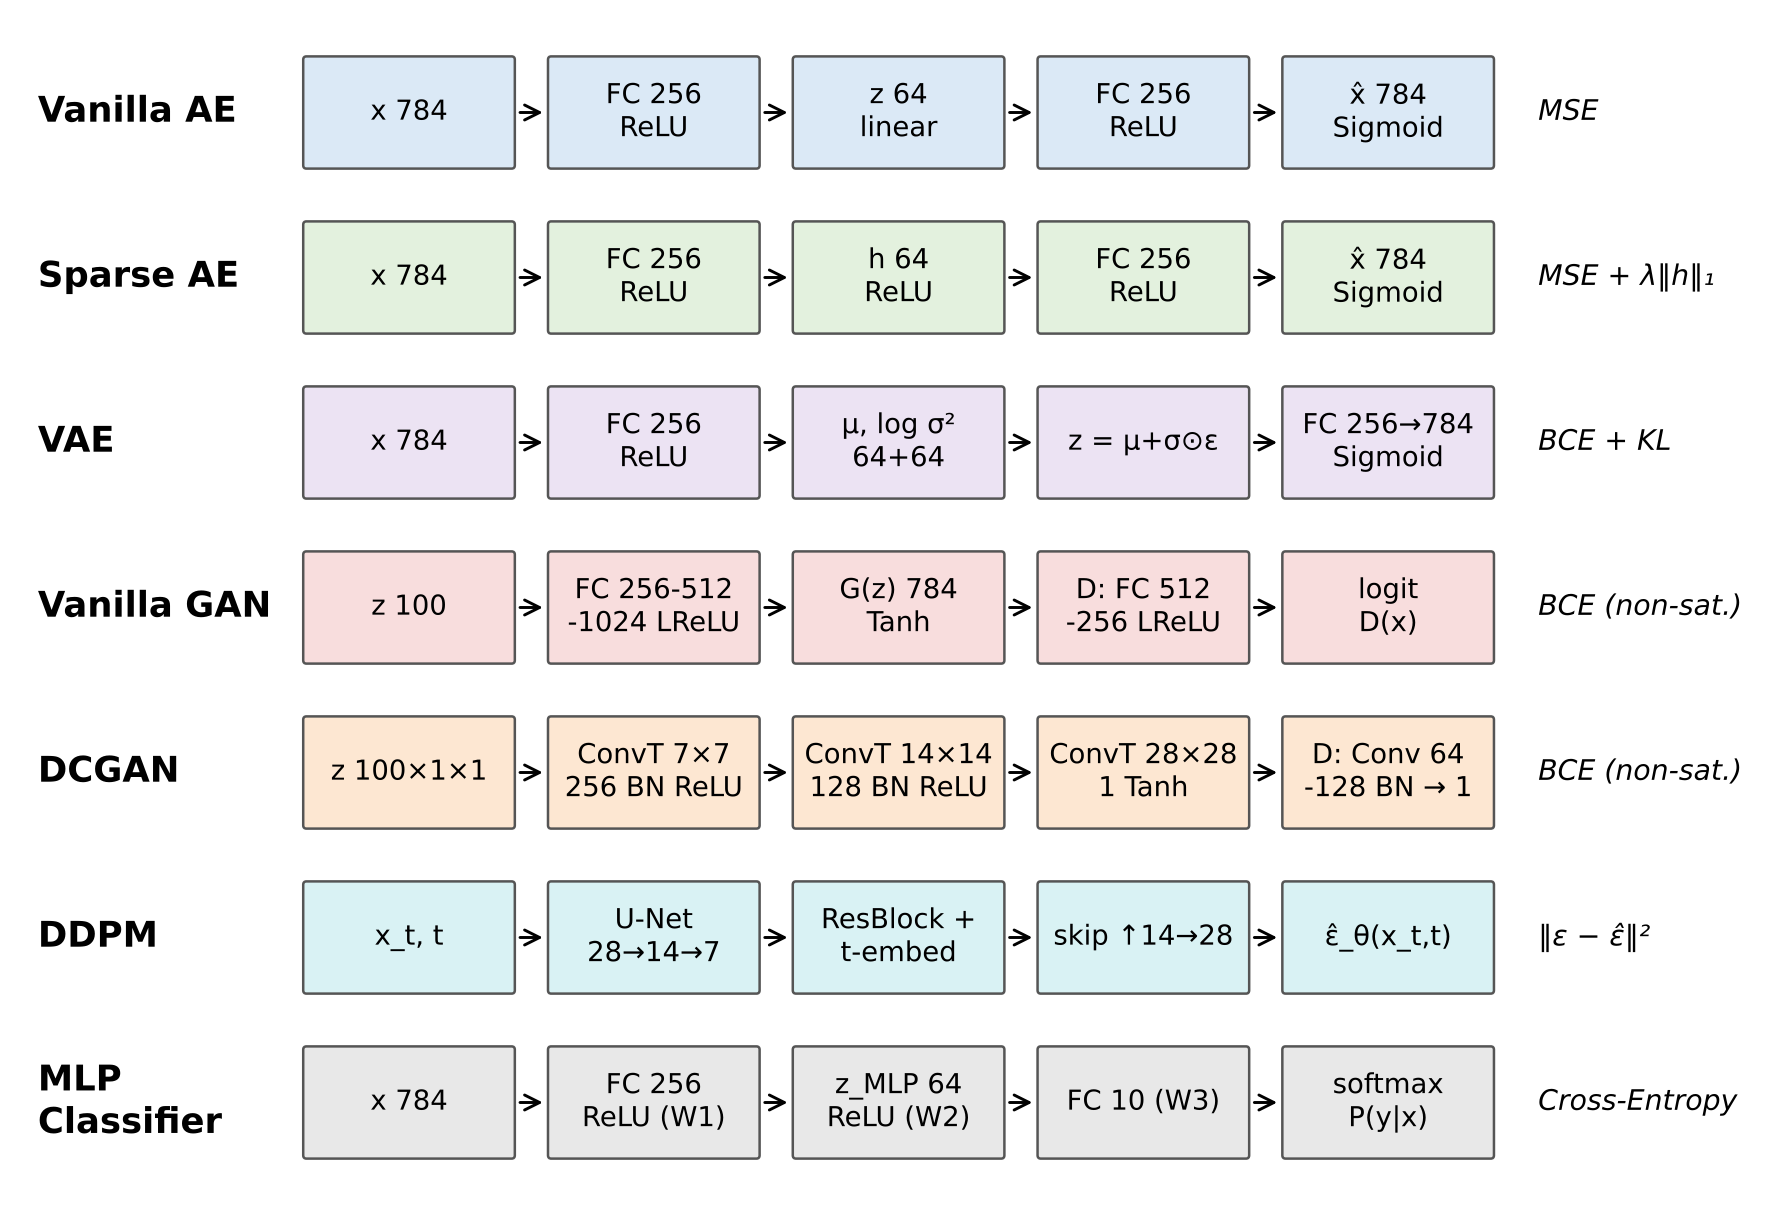
\includegraphics[width=0.93\linewidth]{../outputs/figures/fig0_arsitektur.png}
\caption{\textbf{Figur 0.} Skema arsitektur ketujuh model (blok = lapisan, teks miring = fungsi loss). FC = fully connected,
ConvT = transposed convolution, BN = BatchNorm, LReLU = LeakyReLU(0,2).}
\label{fig:arch}
\end{figure}

\subsection{Tabel konfigurasi parameter}
\begin{table}[h]
\centering\small
\caption{Konfigurasi arsitektur dan optimasi. Jumlah parameter dihitung dari model terlatih.}
\label{tab:config}
\begin{tabular}{@{}lp{4.6cm}cccc@{}}
\toprule
Model & Lapisan & Laten & Aktivasi & Optimizer, LR & Epoch \\
\midrule
Vanilla AE & FC 784-256-64-256-784 & 64 (linear) & ReLU / Sigmoid & Adam, $10^{-3}$ & 30 \\
Sparse AE & idem, $\lambda=10^{-4}$ & 64 (ReLU) & ReLU / Sigmoid & Adam, $10^{-3}$ & 30 \\
VAE & FC 784-256-($\mu$,$\log\sigma^2$)-256-784 & 64 & ReLU / Sigmoid & Adam, $10^{-3}$ & 30 \\
Vanilla GAN & G: FC 100-256-512-1024-784; D: FC 784-512-256-1 & 100 & LReLU / Tanh & Adam, $2\!\cdot\!10^{-4}$, $\beta_1\!=\!0{,}5$ & 50 \\
DCGAN & G: ConvT 7$\times$7$\times$256$\to$14$\times$14$\times$128$\to$28$\times$28; D: Conv 64-128-1 (stride 2) & 100 & ReLU+BN / LReLU / Tanh & Adam, $2\!\cdot\!10^{-4}$, $\beta_1\!=\!0{,}5$ & 20 \\
DDPM & U-Net 3 level (32/64/128), ResBlock+GroupNorm, sinusoidal $t$-embed; $T=1000$, $\beta_t$ linier $10^{-4}\!\to\!0{,}02$, EMA 0,999 & 784 & SiLU & Adam, $2\!\cdot\!10^{-4}$ & 12 \\
MLP Classifier & FC 784-256-64-10 & 64 & ReLU / Softmax & Adam, $10^{-3}$ & 25 \\
\bottomrule
\end{tabular}
\end{table}

\noindent\textbf{Catatan desain.} (i) Uji awal 3 epoch menunjukkan Vanilla AE dengan kode ReLU tanpa penalti
kehilangan $\approx$20/64 unit (\emph{dead units}); karena itu Vanilla AE memakai kode laten linear (representasi padat).
(ii) Sparse AE memakai kode ReLU agar penalti L1 menghasilkan nol eksak; $\lambda=10^{-3}$ membuat seluruh unit mati
(kolaps), sehingga dipilih $\lambda=10^{-4}$. (iii) Generator GAN/DCGAN memakai prior berdimensi 100 dan inisialisasi
DCGAN $\mathcal{N}(0;0{,}02)$.

\subsection{Formulasi matematika fungsi loss}
\textbf{Vanilla AE.} Encoder $f_\phi$ dan decoder $g_\theta$ meminimalkan galat rekonstruksi
\begin{equation}
\mathcal{L}_{\text{AE}}=\frac{1}{N}\sum_{i=1}^{N}\frac{1}{D}\lVert x_i-g_\theta(f_\phi(x_i))\rVert_2^2 .
\end{equation}
\textbf{Sparse AE.} Ditambahkan penalti L1 pada kode $h=\mathrm{ReLU}(f_\phi(x))$:
\begin{equation}
\mathcal{L}_{\text{SAE}}=\mathcal{L}_{\text{AE}}+\lambda\,\frac{1}{N}\sum_i\lVert h_i\rVert_1 ,\qquad \lambda=10^{-4}.
\end{equation}
Penalti L1 adalah relaksasi konveks dari norma $\ell_0$; gradiennya konstan ($\lambda\,\mathrm{sign}(h)$) sehingga
mendorong unit yang kurang berguna tepat ke nol.

\textbf{VAE.} Dengan posterior aproksimasi $q_\phi(z|x)=\mathcal{N}(\mu_\phi(x),\mathrm{diag}\,\sigma^2_\phi(x))$ dan
prior $p(z)=\mathcal{N}(0,I)$, VAE memaksimalkan ELBO $\log p_\theta(x)\ge \mathbb{E}_{q}[\log p_\theta(x|z)]-D_{\text{KL}}(q_\phi(z|x)\Vert p(z))$.
Dengan likelihood Bernoulli dan KL tertutup, loss per sampel:
\begin{equation}
\mathcal{L}_{\text{VAE}}=-\sum_{j=1}^{784}\big[x_j\log\hat{x}_j+(1-x_j)\log(1-\hat{x}_j)\big]
-\frac12\sum_{k=1}^{64}\big(1+\log\sigma_k^2-\mu_k^2-\sigma_k^2\big),
\end{equation}
dengan $z=\mu+\sigma\odot\varepsilon$, $\varepsilon\sim\mathcal{N}(0,I)$ (\emph{reparameterization trick}).

\textbf{Vanilla GAN dan DCGAN.} Generator $G$ dan diskriminator $D$ memainkan permainan minimax
\begin{equation}
\min_G\max_D\;V(D,G)=\mathbb{E}_{x\sim p_{\text{data}}}[\log D(x)]+\mathbb{E}_{z\sim\mathcal{N}(0,I)}[\log(1-D(G(z)))].
\end{equation}
Untuk $D$ optimal $D^*(x)=\frac{p_{\text{data}}(x)}{p_{\text{data}}(x)+p_g(x)}$ sehingga $V(D^*,G)=-\log 4+2\,D_{\text{JS}}(p_{\text{data}}\Vert p_g)$.
Dalam implementasi, $D$ meminimalkan $\mathcal{L}_D=-\mathbb{E}[\log D(x)]-\mathbb{E}[\log(1-D(G(z)))]$ dan $G$ memakai
bentuk \emph{non-saturating} $\mathcal{L}_G=-\mathbb{E}[\log D(G(z))]$ (Goodfellow dkk., 2014). DCGAN memakai loss
yang sama; yang berbeda adalah \emph{inductive bias} arsitekturnya (konvolusi, BatchNorm, strided conv tanpa pooling).

\textbf{DDPM.} Proses maju menambahkan derau Gaussian:
$q(x_t|x_0)=\mathcal{N}(\sqrt{\bar\alpha_t}\,x_0,(1-\bar\alpha_t)I)$ dengan $\alpha_t=1-\beta_t$, $\bar\alpha_t=\prod_{s\le t}\alpha_s$.
Jaringan $\varepsilon_\theta$ dilatih dengan objektif \emph{supervised noise prediction}
\begin{equation}
\mathcal{L}_{\text{simple}}=\mathbb{E}_{t\sim\mathcal{U}\{1..T\},\,x_0,\,\varepsilon\sim\mathcal{N}(0,I)}
\big\lVert\varepsilon-\varepsilon_\theta(\sqrt{\bar\alpha_t}x_0+\sqrt{1-\bar\alpha_t}\,\varepsilon,\;t)\big\rVert_2^2 ,
\end{equation}
dan sampling dilakukan dengan $T=1000$ langkah reverse
$x_{t-1}=\frac{1}{\sqrt{\alpha_t}}\big(x_t-\frac{1-\alpha_t}{\sqrt{1-\bar\alpha_t}}\varepsilon_\theta(x_t,t)\big)+\sigma_t z$,
$\sigma_t^2=\tilde\beta_t=\frac{1-\bar\alpha_{t-1}}{1-\bar\alpha_t}\beta_t$.

\textbf{MLP Classifier.} $p(y|x)=\mathrm{softmax}(W_3\,z_{\text{MLP}}+b_3)$ dengan
$z_{\text{MLP}}=\mathrm{ReLU}(W_2\,\mathrm{ReLU}(W_1x+b_1)+b_2)\in\mathbb{R}^{64}$ dan
$\mathcal{L}_{\text{CE}}=-\frac1N\sum_i\log p(y_i|x_i)$.

\subsection{Metrik evaluasi}
MSE dan PSNR $=10\log_{10}(1/\text{MSE})$ dihitung per citra lalu dirata-rata; SSIM memakai
\texttt{skimage} (\texttt{data\_range}=1). FID $=\lVert\mu_r-\mu_g\rVert^2+\mathrm{Tr}(\Sigma_r+\Sigma_g-2(\Sigma_r\Sigma_g)^{1/2})$
dihitung dari fitur pool3 InceptionV3 (\texttt{pytorch-fid}); citra diduplikasi ke 3 kanal dan di-resize ke 299$\times$299.
Statistik referensi berasal dari 7.000 citra test, dan setiap model dievaluasi dengan \textbf{2.000 sampel}.
Latensi diukur sebagai rata-rata 20 pemanggilan (setelah 3 warm-up) untuk batch 64 sampel pada CPU 2 thread;
DDPM diukur 2 kali untuk 1000 langkah penuh.

\section{Bagian III --- Pembuktian Teoretis dan Empiris Batasan MLP Classifier untuk Image Generation}

\subsection{Uraian matematis}
\textbf{(1) $P(y\mid x)$ berbanding $P(x)$.} Cross-Entropy hanya memaksimalkan $\log p(y|x)$; tidak ada suku yang
menghukum hilangnya informasi tentang $x$ selama label tetap dapat ditebak. Pada rantai Markov
$y\to x\to z_{\text{MLP}}\to\hat{y}$, \emph{data processing inequality} memberi $I(x;z)\le H(x)$ dan
optimum klasifikasi hanya menuntut $I(z;y)=I(x;y)\le H(y)=\log 10\approx 3{,}32$ bit. Representasi minimal-cukup
(\emph{information bottleneck}, $\min I(x;z)-\beta I(z;y)$) karenanya membuang variasi intra-kelas (pose, tekstur, ukuran)
yang justru dibutuhkan untuk merekonstruksi atau mensintesis $x$. Model generatif sebaliknya memodelkan
$p(x)=\int p(x|z)p(z)\,dz$ sehingga \emph{seluruh} variasi $x$ harus terkode.

\textbf{(2) $W^{\top}\neq W^{-1}$ dan ReLU tidak injektif.} $W_1\in\mathbb{R}^{256\times784}$ berrank paling tinggi 256, sehingga
menurut teorema rank--nullity terdapat ruang nol berdimensi $784-256=528$: setiap $x+v$ dengan $v\in\ker W_1$
menghasilkan pra-aktivasi yang sama dan tidak dapat dibedakan. Invers kiri tidak ada; transpos hanya sama dengan invers
bila $W^{\top}W=I$ (kolom ortonormal), padahal bobot terlatih memiliki
$\lVert W_1^{\top}W_1-I\rVert_F/\lVert I\rVert_F=\WoneOrth$ dengan bilangan kondisi \WoneCond. ReLU$(u)=\max(0,u)$ memetakan seluruh
setengah-ruang $u<0$ ke 0; pada test set \ReluOne\ pra-aktivasi lapisan 1 dan \ReluTwo\ lapisan 2 terpotong secara ireversibel.
Akibatnya $W^{\top}$ hanya menghasilkan \emph{superposisi template} baris bobot, bukan citra.

\textbf{(3) Tanpa regularisasi kerapatan $P(z)$.} Tidak ada suku seperti $D_{\text{KL}}(q(z|x)\Vert p(z))$ sehingga
distribusi $z_{\text{MLP}}$ bebas berbentuk apa pun (berkelompok per kelas, \ZeroFrac\ komponennya bernilai nol eksak).
Gaussian diagonal $\mathcal{N}(\mu_z,\mathrm{diag}\,\sigma_z^2)$ tidak menutupi manifold ini: \NegFrac\ komponen sampel
bernilai negatif---nilai yang mustahil dihasilkan ReLU.

\subsection{Hasil eksperimen Tahap 1--5}
\textbf{Tahap 1.} MLP $784\!\to\!256\!\to\!64\!\to\!10$ dilatih 25 epoch (checkpoint terbaik dipilih dari akurasi
validation) dan mencapai \textbf{akurasi test \MLPacc\%} ($\ge$ 88\%). Bobot $W_1,W_2,W_3$ dan $z_{\text{MLP}}$ disimpan.

\begin{table}[h]
\centering\small
\caption{Ringkasan kuantitatif eksperimen batasan MLP Classifier (Test Set, 7.000 citra).}
\label{tab:mlp}
\begin{tabular}{@{}lccccl@{}}
\toprule
Eksperimen & MSE $\downarrow$ & PSNR (dB) $\uparrow$ & SSIM $\uparrow$ & Var. intra-kelas & Keterangan \\
\midrule
T2: $W^{\top}$ dari one-hot $y_c$ (vs citra rata-rata kelas) & \TtwoMSE & \TtwoPSNR & \TtwoSSIM & -- & bercak kabur \\
T3: $W^{\top}$ dari $z_{\text{MLP}}$ & \TthreeMSE & \TthreePSNR & \TthreeSSIM & -- & tidak mirip citra \\
T3: pseudo-invers $W^{+}$ dari $z_{\text{MLP}}$ & \TpinvMSE & \TpinvPSNR & \TpinvSSIM & -- & tetap gagal \\
T4: Frozen decoder dari $z_{\text{MLP}}$ & \FdMSE & \FdPSNR & \FdSSIM & \FdVar & detail hilang \\
T4: Vanilla AE ($z_{\text{AE}}\in\mathbb{R}^{64}$) & \AeMSE & \AePSNR & \AeSSIM & \AeVar & pembanding \\
\bottomrule
\end{tabular}
\end{table}

\textbf{Tahap 2 (transpos dari vektor kelas).} $\hat{x}=\mathrm{Sigmoid}(W_1^{\top}\mathrm{ReLU}(W_2^{\top}\mathrm{ReLU}(W_3^{\top}y_c)))$
menghasilkan pola bercak bertekstur frekuensi tinggi (Gambar~\ref{fig:mlp}, baris 2a). Terhadap citra rata-rata
tiap kelas, SSIM hanya \TtwoSSIM: siluet kelas tidak muncul karena tiap baris $W_1$ adalah \emph{detektor} fitur
diskriminatif (positif dan negatif bercampur), bukan potongan citra.

\textbf{Tahap 3 (transpos dari fitur laten citra uji).} Proyeksi $\mathrm{Sigmoid}(W_1^{\top}\mathrm{ReLU}(W_2^{\top}z_{\text{MLP}}))$
menghasilkan SSIM \TthreeSSIM\ terhadap citra asli. Bahkan pseudo-invers Moore--Penrose $W^{+}$, yang merupakan
solusi kuadrat-terkecil terbaik untuk sistem linear, hanya mencapai SSIM \TpinvSSIM: informasi yang telah dibuang oleh ReLU
dan oleh proyeksi ke ruang berdimensi 64 tidak dapat dipulihkan oleh operasi linear apa pun.

\textbf{Tahap 4 (frozen latent decoding).} Dengan seluruh bobot MLP dibekukan (\texttt{requires\_grad=False}),
decoder $64\!\to\!256\!\to\!784$ yang dilatih 30 epoch dengan MSE (arsitektur dan jumlah epoch identik dengan decoder Vanilla AE)
hanya mencapai PSNR \FdPSNR\ dB dibanding \AePSNR\ dB pada Vanilla AE (MSE \FdAeRatio$\times$ lebih besar).
Rasio varians intra-kelas rekonstruksi terhadap citra asli turun dari \AeVar\ (AE) menjadi \FdVar: decoder hanya
dapat menghasilkan ``prototipe kelas'' karena variasi di dalam kelas sudah tidak ada di $z_{\text{MLP}}$.
Menariknya, akurasi MLP pada rekonstruksi frozen decoder (\FdAcc\%) setara dengan rekonstruksi AE (\AeAcc\%): informasi
\emph{kelas} terjaga sempurna, sedangkan informasi \emph{citra} hilang---bukti langsung efek information bottleneck.

\textbf{Tahap 5 (sampling dari ruang laten MLP).} 2.000 sampel $z_{\text{rand}}\sim\mathcal{N}(\mu_z,\mathrm{diag}\,\sigma_z^2)$
diteruskan ke decoder Tahap 4. Jarak rata-rata sampel ke kode training terdekat adalah \NNrand, sedangkan kode test riil
hanya \NNreal\ (\NNratio$\times$ lebih jauh): sampel jatuh di wilayah kosong. Hasilnya berupa citra kabur campuran
beberapa kelas (Gambar~\ref{fig:mlp}, baris 4); entropi prediksi MLP pada sampel ini \EntMLP\ nat, lebih tinggi daripada
sampel VAE (\EntVAE) dan citra riil (\EntReal), serta distribusi kelasnya timpang (kelas Trouser hanya \TrouserMLP\ dari 2.000).
FID sampel ini adalah \FIDmlp, jauh di atas VAE (\FIDvae).

\begin{figure}[h]
\centering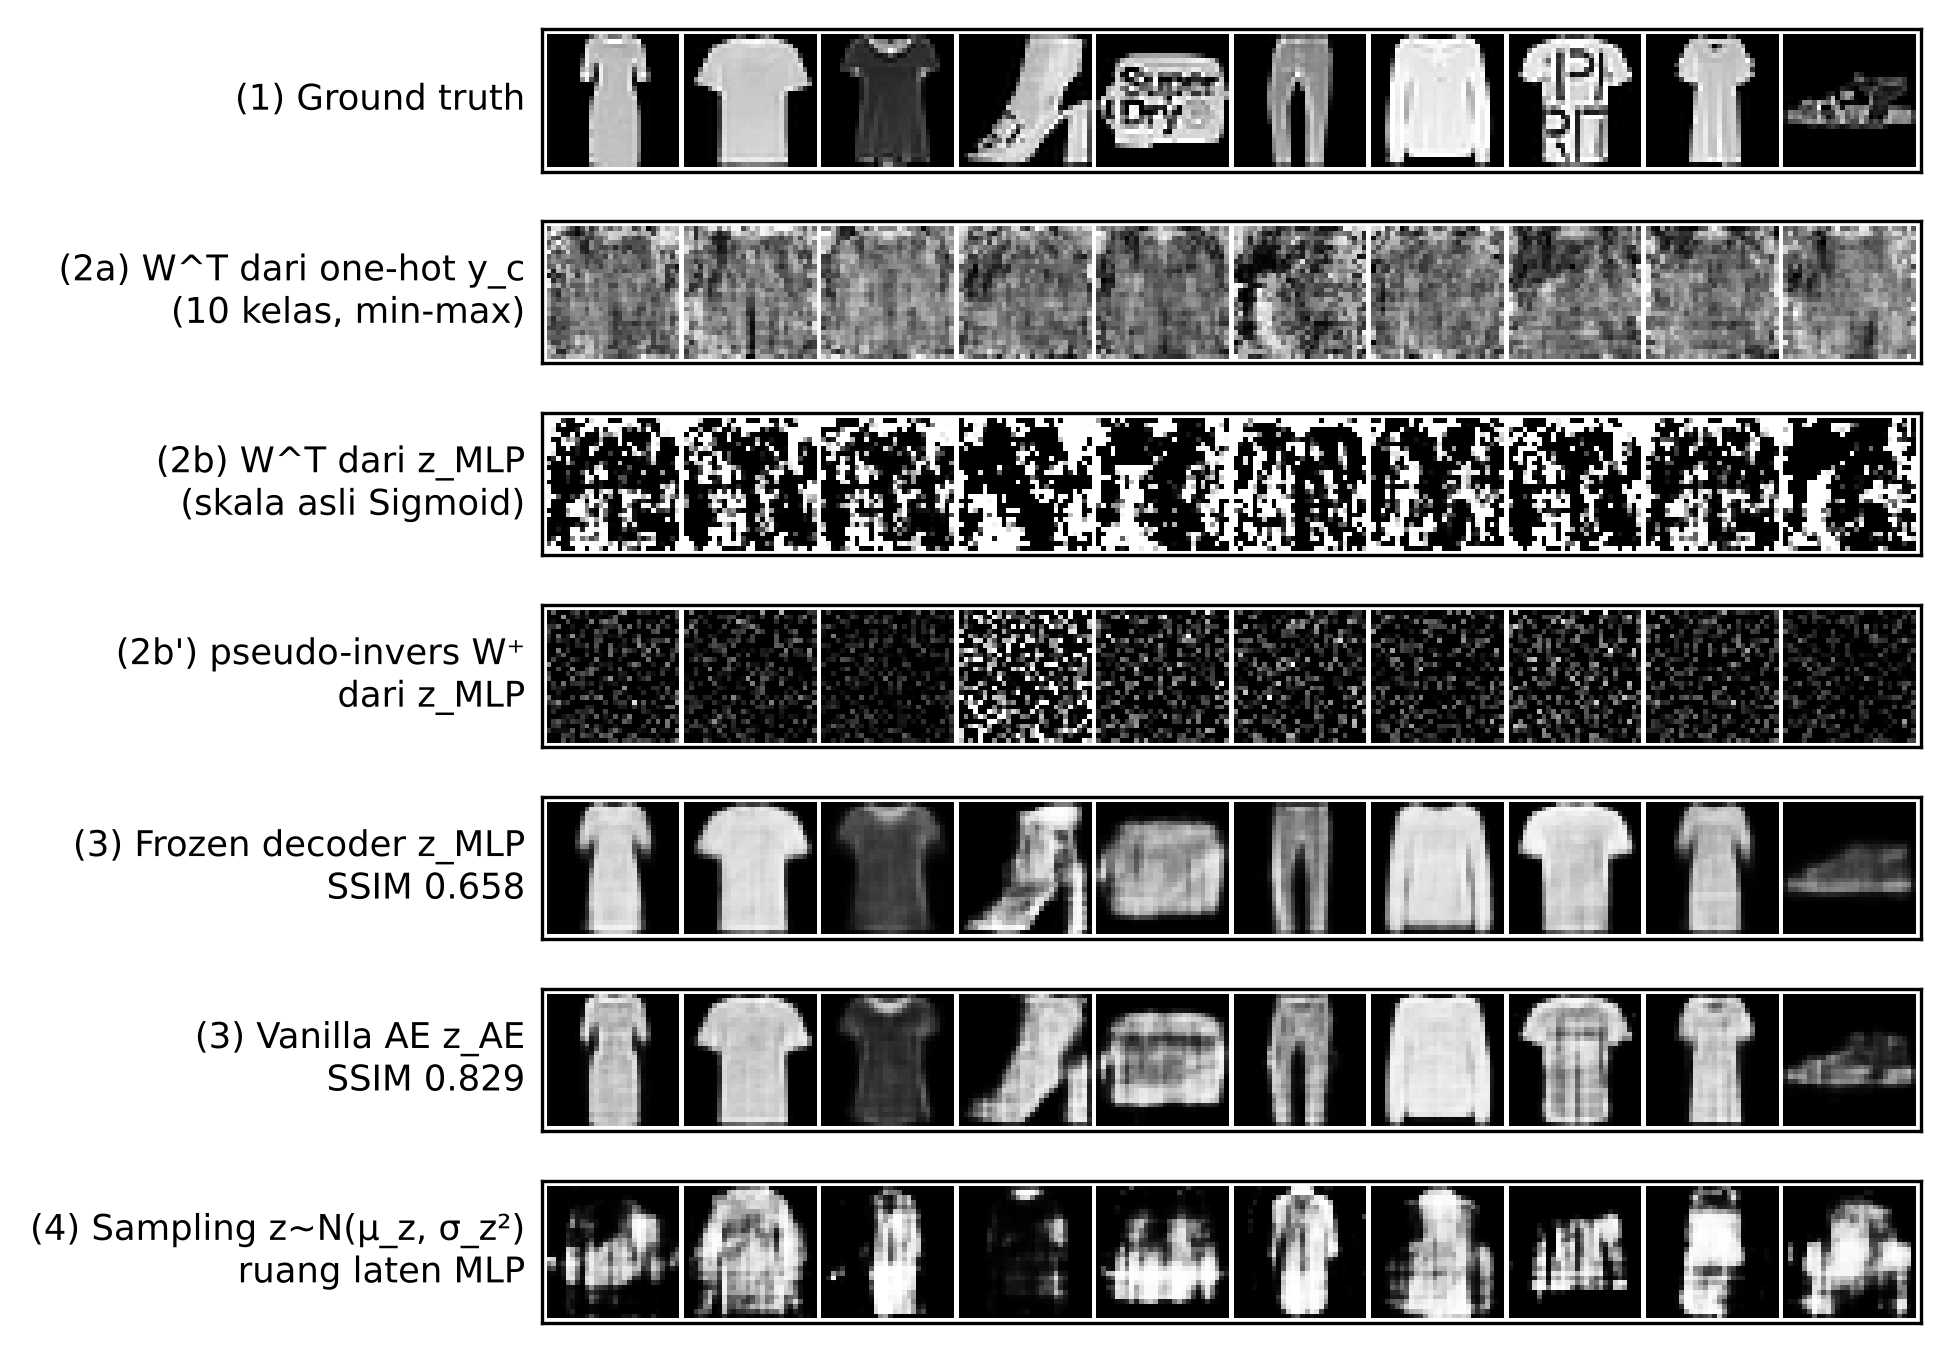
\includegraphics[width=0.92\linewidth]{../outputs/figures/fig3_mlp_batasan.png}
\caption{\textbf{Figur 3.} Bukti empiris batasan MLP Classifier: (1) ground truth; (2a) proyeksi balik $W^{\top}$ dari
one-hot 10 kelas (urutan T-shirt$\to$Ankle boot); (2b) proyeksi balik $W^{\top}$ dari $z_{\text{MLP}}$ (dinormalisasi min-max agar
pola terlihat, lalu dalam skala asli); (3) frozen latent decoder vs Vanilla AE; (4) random prior sampling pada ruang laten MLP.}
\label{fig:mlp}
\end{figure}

\section{Bagian IV --- Tabel Komparasi Metrik Numerik}

\begin{table}[h]
\centering\footnotesize
\setlength{\tabcolsep}{3.2pt}
\caption{Kompilasi kuantitatif pada Test Set (7.000 citra). Training time = rata-rata detik per epoch (CPU, 1 thread);
latensi = ms per batch 64 sampel (CPU, 2 thread; AE/SAE: rekonstruksi, VAE/GAN/DCGAN/DDPM: sintesis dari prior).
FID: 2.000 sampel vs statistik 7.000 citra test (FID citra riil validation vs test = \FIDreal).}
\label{tab:main}
\begin{tabular}{@{}lccccccccp{3.0cm}@{}}
\toprule
Arsitektur & Dim laten & Param (M) & Train/epoch (s) & Latensi (ms) & MSE $\downarrow$ & PSNR (dB) $\uparrow$ & SSIM $\uparrow$ & FID $\downarrow$ & Kestabilan training \\
\midrule
Vanilla AE & 64 & \PAE & \TAE & \LAE & \MSEAE & \PSNRAE & \SSIMAE & N/A (latent voids) & Stabil, konvergen monoton \\
Sparse AE & 64 (ReLU, L1) & \PSAE & \TSAE & \LSAE & \MSESAE & \PSNRSAE & \SSIMSAE & N/A (latent voids) & Stabil, konvergen monoton \\
VAE & 64 & \PVAE & \TVAE & \LVAE & \MSEVAE & \PSNRVAE & \SSIMVAE & \FIDVAE & Stabil, konvergen \\
Vanilla GAN & 100 (prior) & \PGAN & \TGAN & \LGAN & N/A & N/A & N/A & \FIDGAN & Equilibrium semu $D\!\approx\!0{,}5$; sampel berbintik \\
DCGAN & 100 (prior) & \PDCGAN & \TDCGAN & \LDCGAN & N/A & N/A & N/A & \FIDDCGAN & Cukup stabil, osilasi $\mathcal{L}_G$ lebih besar \\
DDPM & 28$\times$28 & \PDDPM & \TDDPM & \LDDPM & N/A & N/A & N/A & \FIDDDPM & Sangat stabil, loss turun monoton \\
\bottomrule
\end{tabular}
\end{table}

\begin{table}[h]
\centering\footnotesize
\caption{Metrik pendukung. \emph{Coverage} = entropi ternormalisasi distribusi kelas sampel menurut MLP Classifier
(1 = 10 kelas merata; citra riil = \COVreal). Gaussian-fit = sampling $z\sim\mathcal{N}(\mu_z,\mathrm{diag}\,\sigma_z^2)$
pada ruang laten model deterministik.}
\label{tab:aux}
\begin{tabular}{@{}lcccc|lcc@{}}
\toprule
Model generatif & FID & Coverage & Kelas min/maks & & Pembanding & FID & Coverage \\
\midrule
VAE & \FIDVAE & \COVVAE & \MINCVAE/\MAXCVAE & & Vanilla AE Gaussian-fit & \FIDaegauss & \COVAEgauss \\
Vanilla GAN & \FIDGAN & \COVGAN & \MINCGAN/\MAXCGAN & & Sparse AE Gaussian-fit & \FIDsaegauss & \COVSAEgauss \\
DCGAN & \FIDDCGAN & \COVDCGAN & \MINCDCGAN/\MAXCDCGAN & & Laten MLP Classifier (T5) & \FIDmlp & \COVmlp \\
DDPM & \FIDDDPM & \COVDDPM & \MINCDDPM/\MAXCDDPM & & Citra riil (val) & \FIDreal & \COVreal \\
\bottomrule
\end{tabular}
\end{table}

\textbf{Sparsitas kode.} Vanilla AE: \ZFAE\ komponen kode bernilai nol, \ACTAE\ unit aktif per sampel, \DEADAE\ unit mati.
Sparse AE: \ZFSAE\ nol, hanya \ACTSAE\ dari 64 unit aktif per sampel, \DEADSAE\ unit tidak pernah aktif di test set.
DDPM membutuhkan \LDDPMstep\ ms untuk \emph{satu} langkah denoising batch 64, sehingga 1000 langkah
$\approx$\DDPMxGAN$\times$ lebih lambat daripada satu forward pass generator DCGAN.

\textbf{Catatan pengukuran.} FID dengan $N=2.000$ bias ke atas dibanding protokol standar $N=50.000$ dan citra 28$\times$28
di-upscale ke 299$\times$299, sehingga angka absolut tidak dapat dibandingkan langsung dengan literatur. Namun seluruh model
memakai $N$, referensi, dan pra-pemrosesan yang sama, sehingga \emph{urutan} antarmodel valid. Training time diukur saat dua
proses berjalan paralel pada 2 core (masing-masing 1 thread), sedangkan latensi diukur saat mesin tidak menjalankan proses lain.

\section{Bagian V --- Kompilasi Lima Visualisasi Komparatif Utama}
Figur 3 telah disajikan pada Bagian III (Gambar~\ref{fig:mlp}). Seluruh figur dibuat dari Test Set dan sampel ber-seed tetap.

\begin{figure}[H]
\centering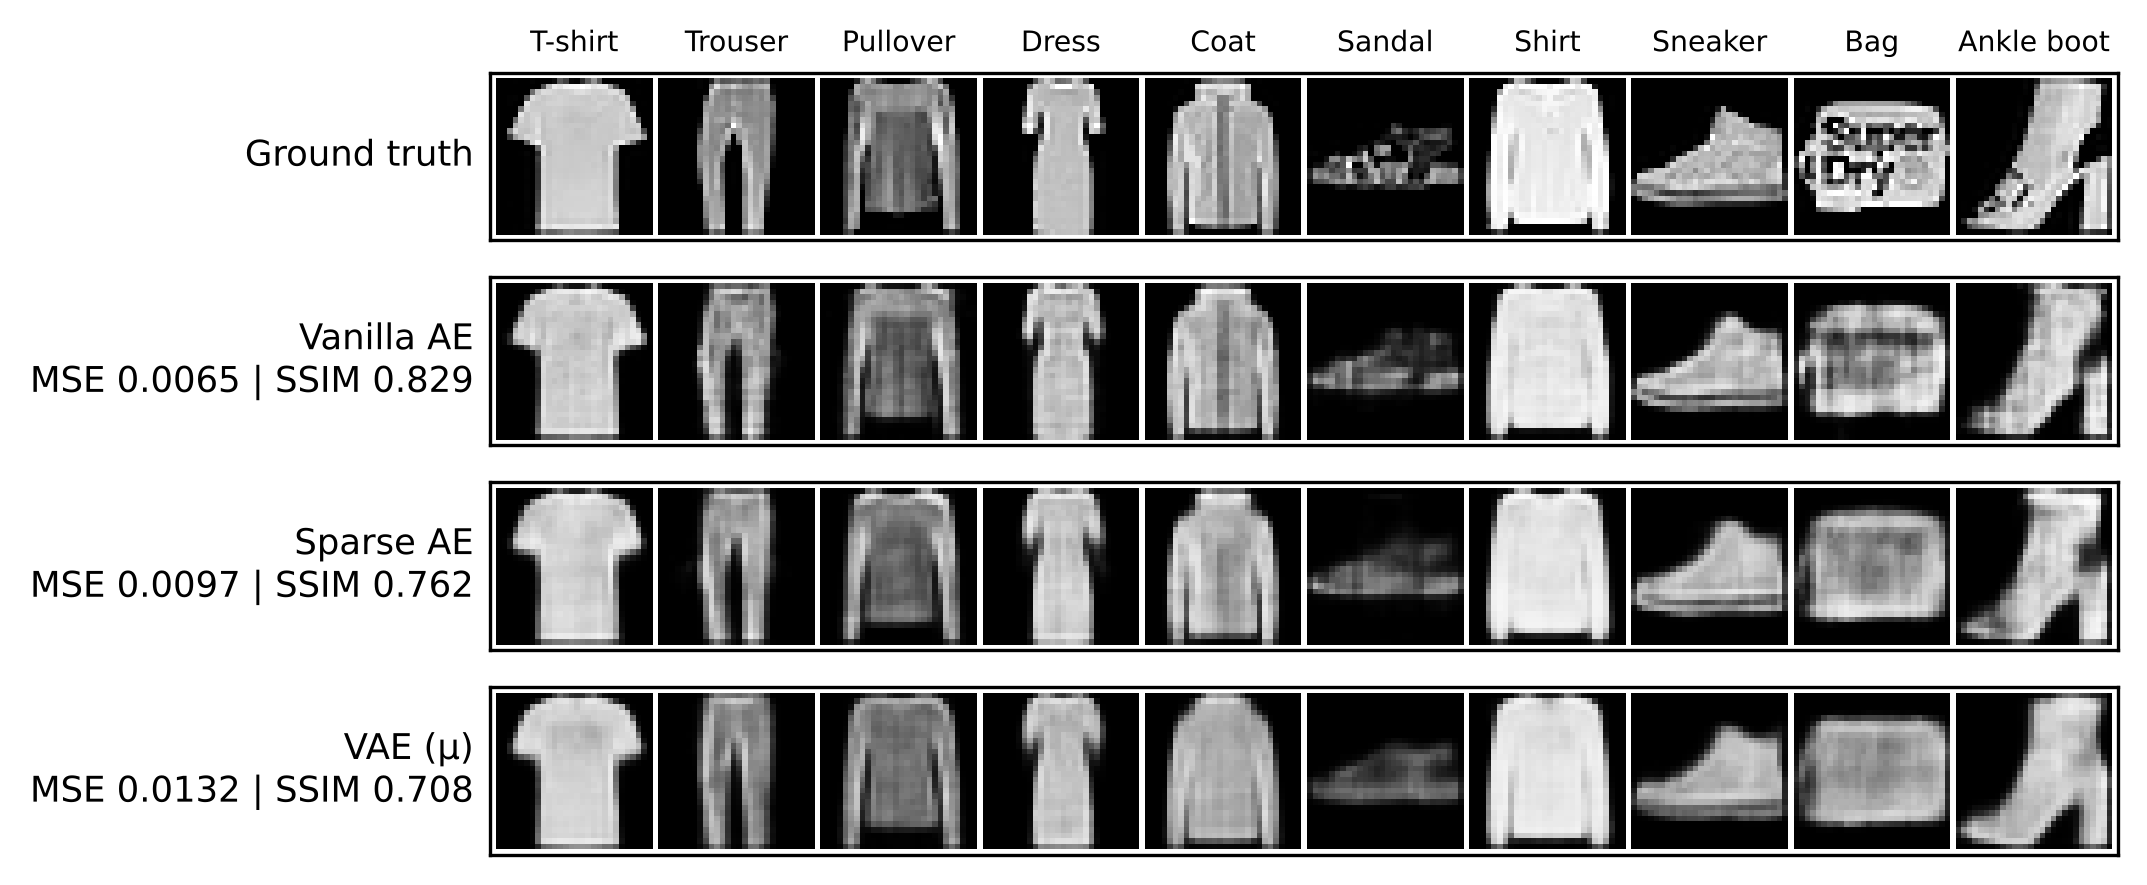
\includegraphics[width=0.95\linewidth]{../outputs/figures/fig1_rekonstruksi.png}
\caption{\textbf{Figur 1.} Rekonstruksi side-by-side satu citra test per kelas (kiri ke kanan: T-shirt $\to$ Ankle boot).
Baris: ground truth, Vanilla AE, Sparse AE, VAE (decode $\mu$).}
\label{fig:recon}
\end{figure}

\textbf{Analisis Figur 1.} Ketiga model mempertahankan siluet global, tetapi berbeda pada detail frekuensi tinggi.
Vanilla AE (kode padat, semua 64 unit aktif) paling banyak mempertahankan pola lokal---garis tali sandal, motif kaos,
dan tepi sepatu---sehingga SSIM-nya tertinggi (\SSIMAE). Sparse AE hanya mengaktifkan $\approx$\ACTSAE\ unit per citra:
kode berperilaku seperti kombinasi sedikit ``bagian'' (\emph{parts}) sehingga motif halus diganti tekstur generik dan
tepi sedikit melunak (SSIM \SSIMSAE). VAE paling buram (SSIM \SSIMVAE): selain loss piksel, suku KL memaksa posterior
$q(z|x)$ tiap citra melebar dan saling tumpang tindih, sehingga decoder belajar mengeluarkan rata-rata dari beberapa citra
yang berbagi wilayah laten yang sama. Detail seperti tulisan pada tas dan pola kotak-kotak hilang paling dulu.

\begin{figure}[H]
\centering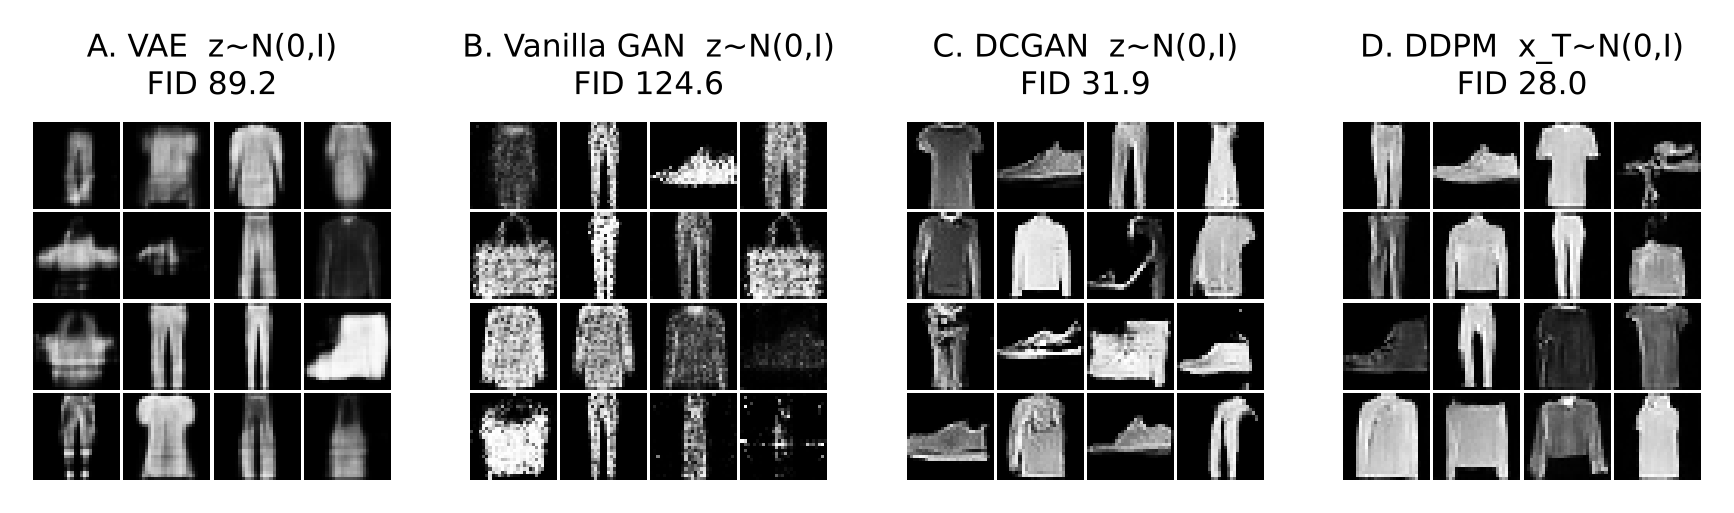
\includegraphics[width=\linewidth]{../outputs/figures/fig2_sampling.png}
\caption{\textbf{Figur 2.} Random generative sampling 4$\times$4 dari prior $\mathcal{N}(0,I)$: (A) VAE, (B) Vanilla GAN,
(C) DCGAN, (D) DDPM (reverse diffusion 1000 langkah dari $x_T\sim\mathcal{N}(0,I)$). Angka = FID (2.000 sampel).}
\label{fig:samples}
\end{figure}

\textbf{Analisis Figur 2.} \FigTwoText

\begin{figure}[H]
\centering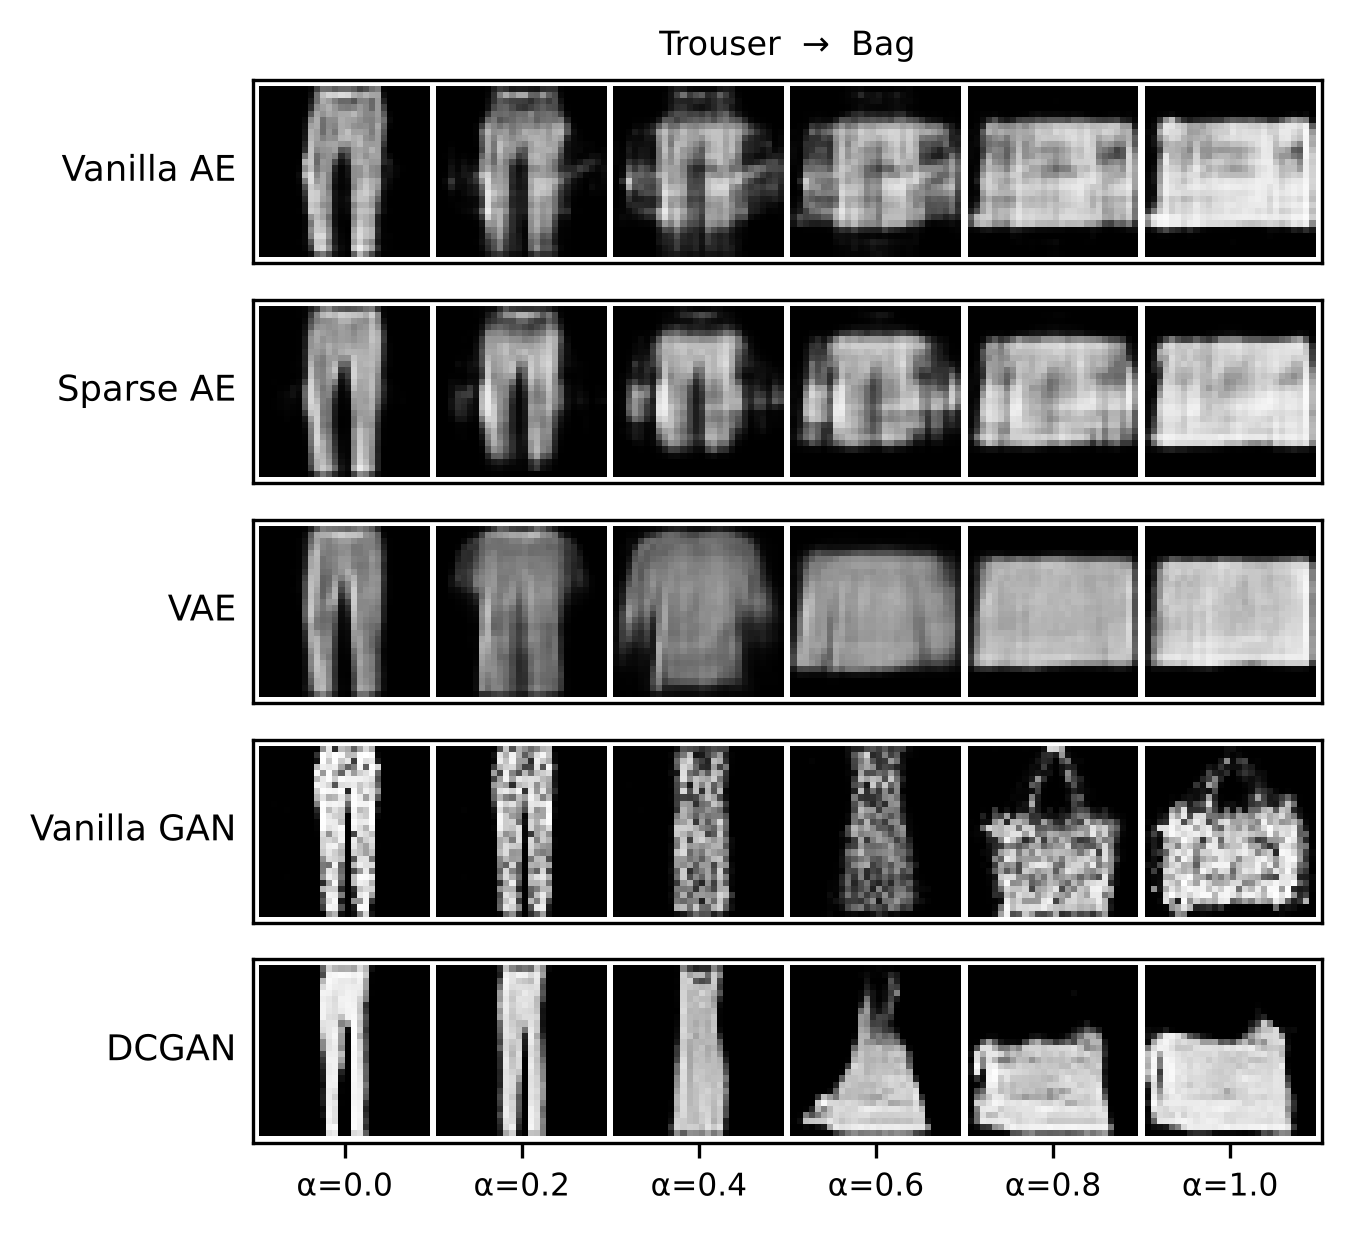
\includegraphics[width=0.66\linewidth]{../outputs/figures/fig4_interpolasi.png}
\caption{\textbf{Figur 4.} Interpolasi laten linier $z(\alpha)=(1-\alpha)z_A+\alpha z_B$ dari Trouser ke Bag.
AE/Sparse AE/VAE: $z_A,z_B$ = kode encoder dua citra test (VAE memakai $\mu$). GAN/DCGAN tidak memiliki encoder,
sehingga $z_A,z_B$ dipilih dari 5.000 vektor prior acak yang hasilnya diklasifikasikan MLP sebagai Trouser/Bag dengan
probabilitas tertinggi (keduanya $\approx$1,0).}
\label{fig:interp}
\end{figure}

\textbf{Analisis Figur 4.} Pada Vanilla AE dan Sparse AE, titik tengah ($\alpha=0{,}4$--$0{,}6$) berupa \emph{superposisi}
dua siluet---kaki celana tampak ``menembus'' badan tas, disertai pita-pita horizontal dan bercak kotak. Ini bukan objek
yang valid. Jarak titik tengah ke kode training terdekat (dinormalisasi terhadap kode test riil) mencapai
\VOIDAE$\times$ untuk Vanilla AE dan \VOIDSAE$\times$ untuk Sparse AE: lintasan lurus melewati wilayah laten yang
tidak pernah dilihat decoder. VAE berperilaku lain: transisinya halus dan setiap titik antara adalah pakaian yang masuk akal
(celana $\to$ atasan berlengan $\to$ tas), dengan rasio jarak terkecil (\VOIDVAE$\times$). Suku KL menarik seluruh posterior
ke dekat $\mathcal{N}(0,I)$ sehingga wilayah di antara dua kode terisi oleh posterior citra lain. GAN dan DCGAN juga
menghasilkan transisi semantik (celana $\to$ dress $\to$ tas) karena generator dilatih memetakan \emph{seluruh} massa prior
ke citra realistis; perbedaannya, Vanilla GAN tetap membawa derau bintik di setiap frame, sedangkan DCGAN bersih.

\begin{figure}[H]
\centering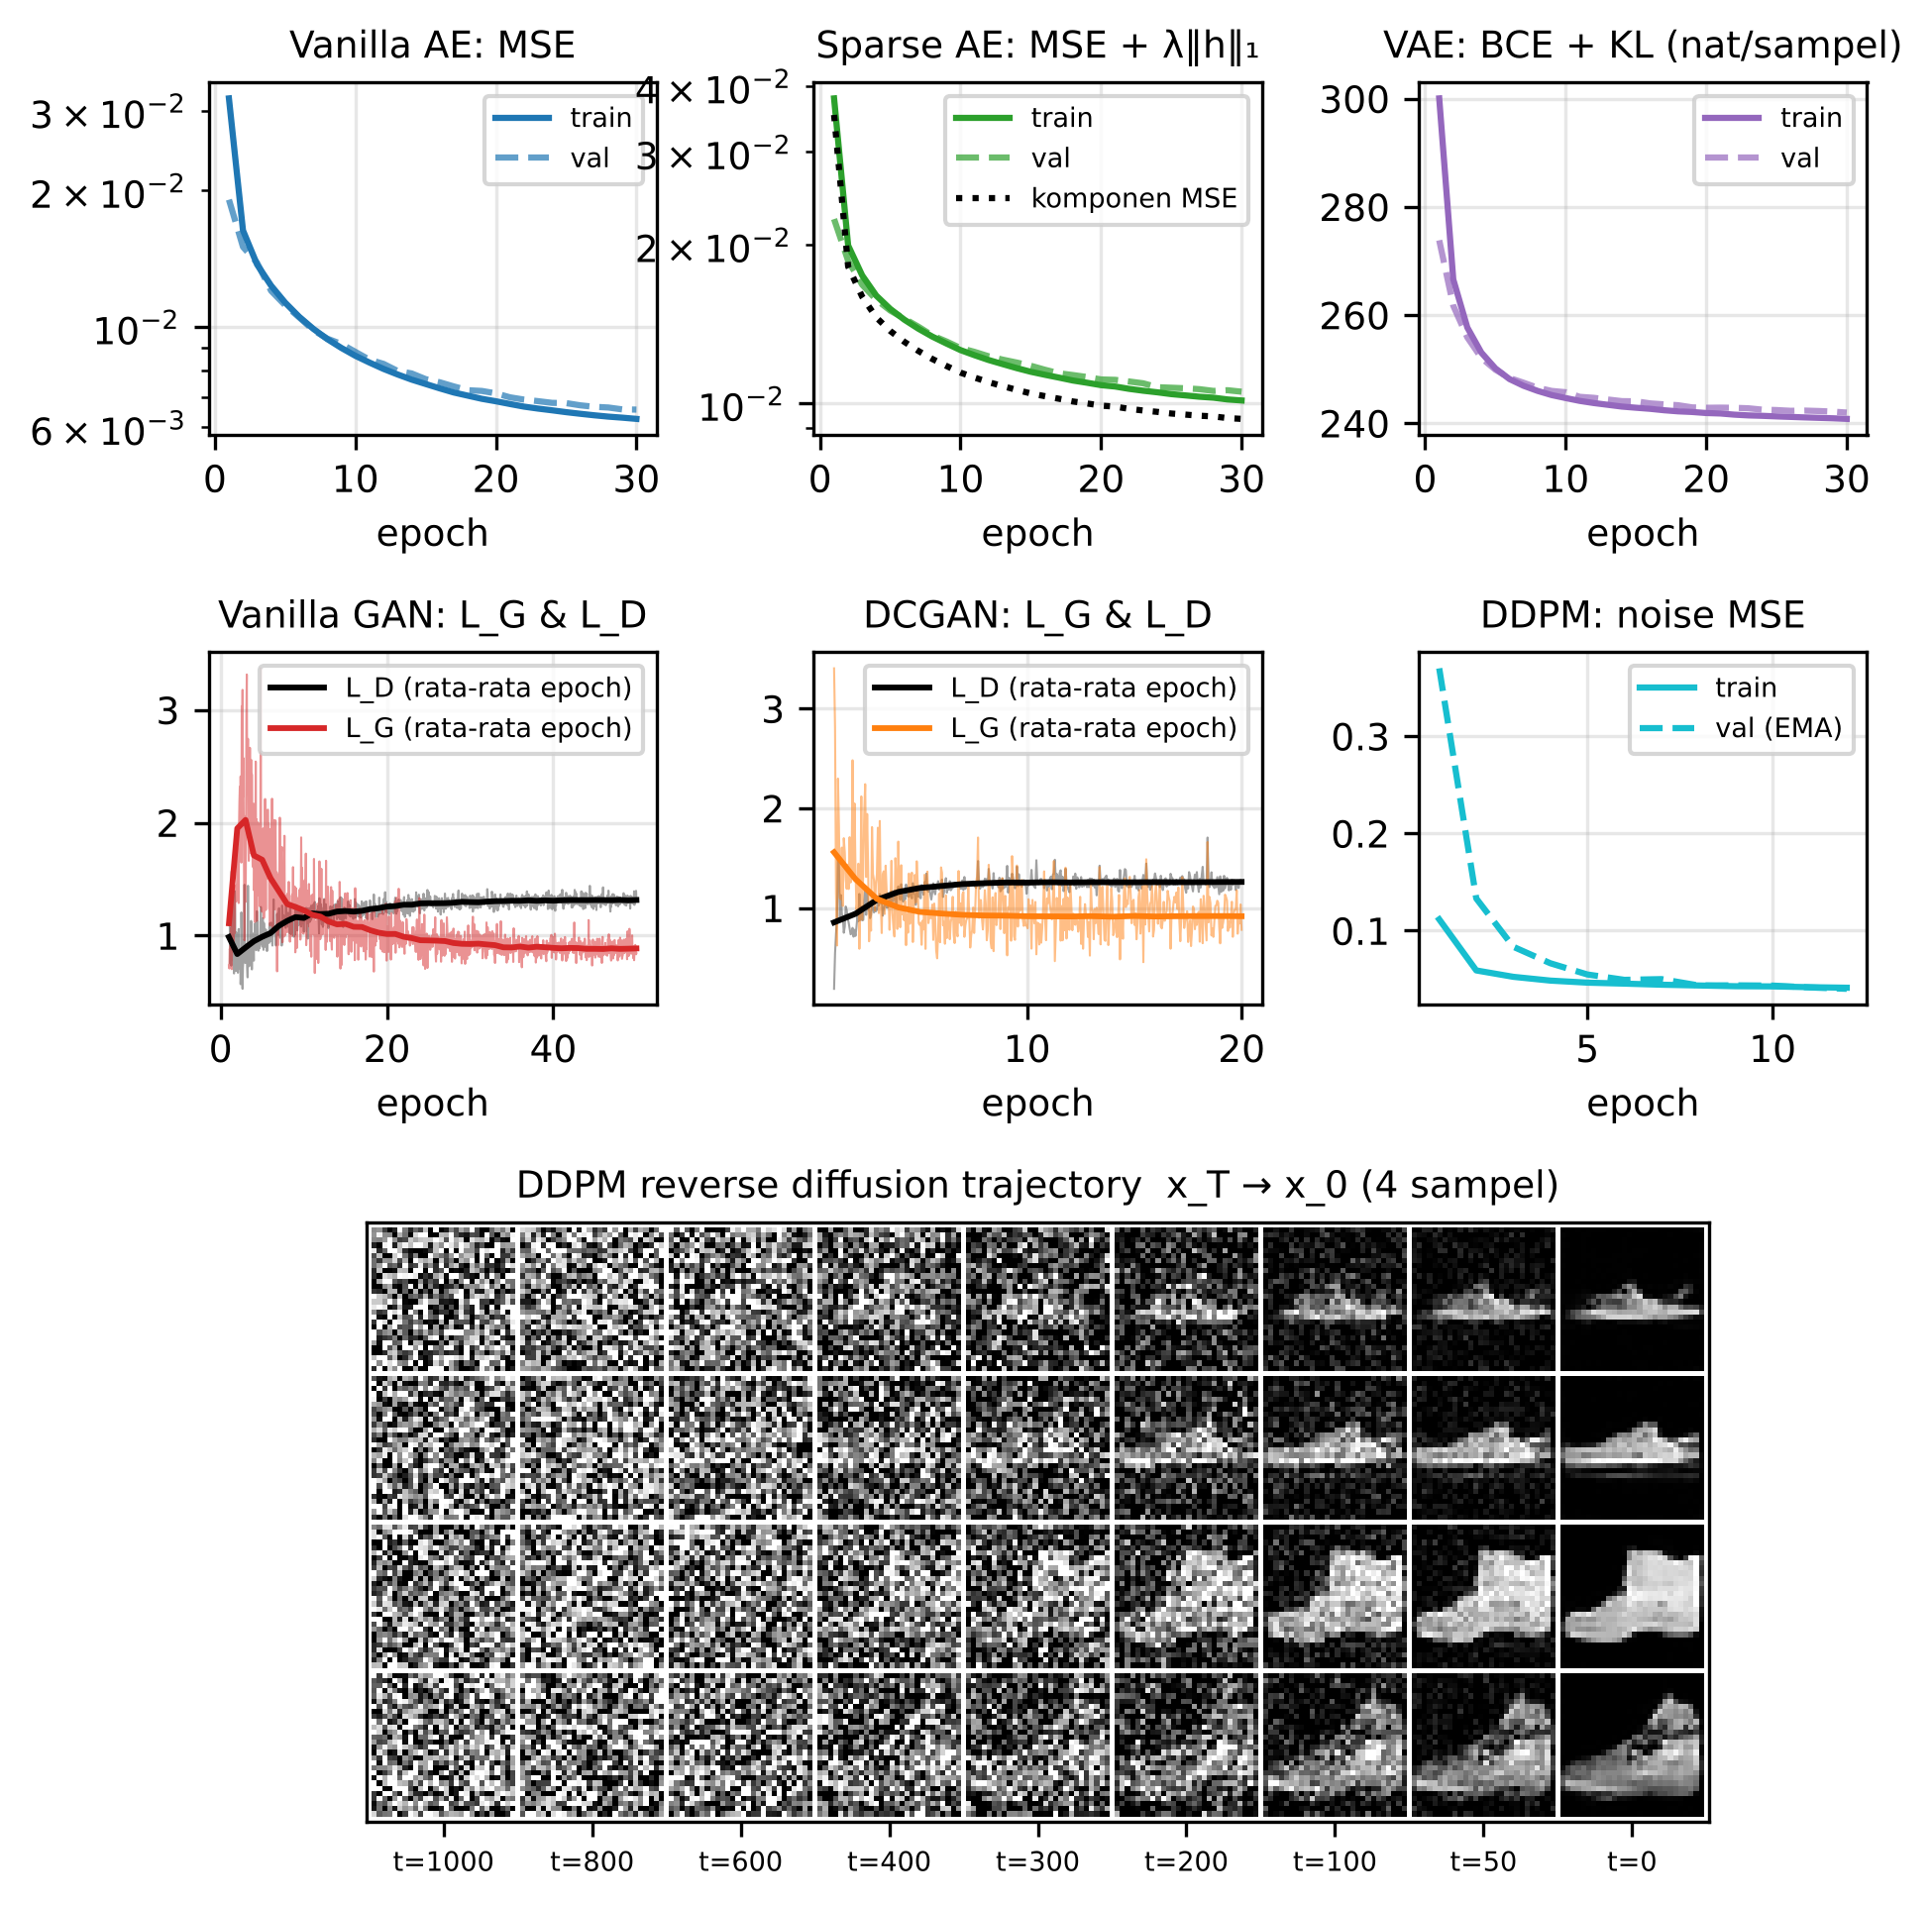
\includegraphics[width=\linewidth]{../outputs/figures/fig5_loss_ddpm.png}
\caption{\textbf{Figur 5.} Atas: kurva loss AE (MSE), Sparse AE (total dan komponen MSE), VAE (negatif ELBO, nat/sampel).
Tengah: loss $G$ dan $D$ Vanilla GAN dan DCGAN (garis tipis = setiap 20 iterasi, tebal = rata-rata epoch) serta noise-prediction
loss DDPM. Bawah: trajektori reverse diffusion DDPM $x_T\to x_0$.}
\label{fig:loss}
\end{figure}

\textbf{Analisis Figur 5.} Ketiga autoencoder turun monoton dengan selisih train--val kecil (Vanilla AE akhir: train
\AEtrain, val \AEval). Pada Sparse AE, komponen MSE turun lebih lambat daripada AE karena sebagian gradien dipakai untuk
menekan $\lVert h\rVert_1$. Kedua GAN tidak pernah ``konvergen'' dalam arti loss menuju nol: $\mathcal{L}_D$ naik
mendekati $2\log 2\approx1{,}39$ dan $\mathcal{L}_G$ turun mendekati $\log 2\approx0{,}69$, yaitu kondisi
$D(x)\approx D(G(z))\approx0{,}5$ (akhir Vanilla GAN: $D(x)=\DRGAN$, $D(G(z))=\DFGAN$; DCGAN: \DRDCGAN/\DFDCGAN).
Fluktuasi $\mathcal{L}_G$ per iterasi pada paruh akhir training lebih besar pada DCGAN (std \GSTDDCGAN) daripada Vanilla GAN
(std \GSTDGAN). DDPM turun mulus dari \DDPMfirst\ ke \DDPMlast\ (val EMA \DDPMval) tanpa osilasi. Trajektori bawah
memperlihatkan siluet kasar muncul pertama kali sekitar $t\approx300$--$200$ dan detail tekstur terbentuk pada $t<100$:
proses generasi berlangsung dari frekuensi rendah ke tinggi (\emph{coarse-to-fine}).

\section{Bagian VI --- Pembahasan Kritis, Jawaban Pertanyaan Penelitian, dan Rekomendasi}

\subsection*{Q1 --- Reconstruction fidelity vs generative quality}
\textbf{Rekonstruksi.} Urutan fidelitas pada test set adalah Vanilla AE (MSE \MSEAE, PSNR \PSNRAE\ dB, SSIM \SSIMAE)
$>$ Sparse AE (\MSESAE; \PSNRSAE\ dB; \SSIMSAE) $>$ VAE (\MSEVAE; \PSNRVAE\ dB; \SSIMVAE). Penalti $\lambda\lVert h\rVert_1$
menurunkan PSNR sekitar \PSNRdropSAE\ dB karena memaksa trade-off: setiap unit yang aktif ``membayar'' biaya $\lambda$, sehingga
optimum menutup unit dengan kontribusi rekonstruksi kecil (hanya \ACTSAE\ dari 64 unit aktif per citra, \DEADSAE\ unit tidak
pernah aktif). Kapasitas efektif kode turun, dan detail halus---yang hanya sedikit menurunkan MSE---adalah yang pertama
dikorbankan. Vanilla AE tidak memiliki biaya tersebut sehingga memakai seluruh 64 dimensi secara padat. VAE paling rendah
karena ELBO menyeimbangkan rekonstruksi dengan KL ($\approx$\KLVAE\ nat/sampel): kode dibuat berderau dan ditarik ke
$\mathcal{N}(0,I)$, sehingga informasi yang bisa dibawa $z$ dibatasi (rate--distortion).

\textbf{Generasi dari prior.} \QoneFID\ Urutan ini terbalik dibandingkan rekonstruksi: VAE kalah dalam fidelitas tetapi
merupakan satu-satunya autoencoder yang dapat disampling. Vanilla AE yang disampling dengan Gaussian-fit mendapat FID
\FIDaegauss\ (Sparse AE \FIDsaegauss), jauh lebih buruk dari VAE, karena kode AE tidak pernah dipaksa mengisi prior.

\subsection*{Q2 --- Blurriness vs sharp edges dan representasi fitur}
Untuk decoder deterministik $\hat{x}=g(z)$, minimisasi MSE memiliki solusi optimal $g^*(z)=\mathbb{E}[x\mid z]$.
Jika satu $z$ bersesuaian dengan beberapa citra yang mungkin (karena bottleneck 64-d membuang sebagian informasi, atau karena
derau posterior VAE), decoder optimal mengeluarkan \emph{rata-rata} mereka. Rata-rata beberapa tepi yang sedikit bergeser
adalah gradasi lembut, yaitu blur. BCE pada VAE berperilaku sama karena estimasi maksimum likelihood Bernoulli per piksel
juga menghasilkan $\mathbb{E}[x_j\mid z]$, dan likelihood yang faktorial per piksel tidak dapat menyatakan bahwa ``tepi ada di
posisi A \emph{atau} B, bukan setengah di keduanya''. GAN tidak memiliki target piksel: generator dihukum jika $D$ dapat
membedakan $G(z)$ dari data, sehingga meminimalkan (secara aproksimasi) $D_{\text{JS}}(p_{\text{data}}\Vert p_g)$. Citra rata-rata
yang buram berada di luar support $p_{\text{data}}$, sehingga mudah dikenali $D$. Divergensi ini \emph{mode-seeking}: generator
didorong memilih satu mode yang tajam daripada rata-rata banyak mode. Inilah sebabnya DCGAN menghasilkan kontur tajam
(Gambar~\ref{fig:samples}C). Vanilla GAN memang tajam, tetapi derau bintiknya menunjukkan sisi lain: $D$ berbasis MLP tidak
dapat mendeteksi inkonsistensi lokal antarpiksel, sehingga $G$ tidak pernah dihukum karenanya (lihat Q3).

\textbf{Struktur fitur Sparse AE vs Vanilla AE.} Pada Vanilla AE, \ZFAE\ komponen kode bernilai nol (kode linear, padat):
setiap citra dikodekan sebagai kombinasi \emph{semua} arah laten, dan informasi tersebar (\emph{distributed}). Pada Sparse AE,
\ZFSAE\ komponen bernilai nol eksak. Setiap citra hanya memakai $\approx$\ACTSAE\ unit, sehingga unit cenderung terspesialisasi
menjadi detektor ``bagian'' (siluet atasan, sol sepatu, pegangan tas) yang dapat dijumlahkan. Representasi ini lebih mudah
diinterpretasi dan lebih tahan derau, tetapi dengan bottleneck 64 dimensi biaya fidelitasnya terlihat jelas pada Q1.

\subsection*{Q3 --- Stabilitas training, dinamika arsitektur, dan Generative Trilemma}
\textbf{Vanilla GAN vs DCGAN.} Secara teori, minimax asli menyebabkan \emph{vanishing gradient}: jika $D$ terlalu kuat,
$D(G(z))\to0$ dan $\nabla_G\log(1-D(G(z)))\to0$. Selain itu, jika support $p_g$ dan $p_{\text{data}}$ hampir tidak beririsan,
$D_{\text{JS}}$ jenuh di $\log2$ dan tidak memberi arah. \emph{Mode collapse} terjadi ketika $G$ menemukan satu keluaran
yang menipu $D$ saat itu dan memetakan banyak $z$ ke sana. Dalam eksperimen ini, kedua GAN memakai loss non-saturating dan
Adam $\beta_1=0{,}5$. Hasilnya, \textbf{tidak ada mode collapse tingkat kelas}: coverage Vanilla GAN \COVGAN\ dan DCGAN \COVDCGAN,
setara citra riil (\COVreal). Kegagalan Vanilla GAN muncul dalam bentuk lain, yaitu \emph{equilibrium semu}: $D(x)$ dan
$D(G(z))$ mendekati 0,5 (\DRGAN/\DFGAN) dan norma gradien $G$ menurun dari \GNGANfirst\ menjadi \GNGANlast, padahal sampel
masih berbintik (FID \FIDGAN). $D$ berbasis MLP memperlakukan 784 piksel sebagai vektor tanpa struktur spasial, sehingga
$D$ tidak dapat membedakan derau lokal. Akibatnya sinyal gradien ke $G$ melemah sebelum kualitas tercapai; ini adalah bentuk
praktis \emph{vanishing learning signal}. DCGAN memitigasinya melalui prinsip Radford dkk.:
(1) konvolusi berbagi bobot dan lokal, sehingga $D$ peka terhadap tepi dan tekstur, dan $G$ menghasilkan piksel tetangga yang
berkorelasi; (2) strided (transposed) convolution tanpa pooling; (3) BatchNorm di $G$ dan $D$ yang menstabilkan skala aktivasi
dan aliran gradien; (4) ReLU di $G$ dan LeakyReLU di $D$ sehingga gradien tidak mati; (5) inisialisasi $\mathcal{N}(0;0{,}02)$.
Hasilnya FID turun \GANoverDCGAN$\times$ (\FIDGAN$\to$\FIDDCGAN). Menariknya, loss $G$ per iterasi DCGAN justru lebih fluktuatif
(std \GSTDDCGAN\ vs \GSTDGAN). Osilasi ini tanda $D$ yang \emph{informatif}, bukan ketidakstabilan, sehingga kurva loss GAN tidak
dapat dipakai sebagai indikator kualitas.

\textbf{GAN vs DDPM.} DDPM meminimalkan regresi MSE terhadap target tetap $\varepsilon$ untuk $t$ acak. Objektifnya adalah
masalah optimasi tunggal (bukan permainan dua pemain) dan landskapnya tidak berubah selama training. Kurva loss DDPM turun
monoton tanpa osilasi (\DDPMfirst$\to$\DDPMlast), dan val loss ber-EMA mengikuti train loss.

\textbf{Trilemma.} \TrilemmaText

\subsection*{Q4 --- Struktur latent space dan interpolasi}
Seperti terlihat pada Gambar~\ref{fig:interp}, Vanilla AE dan Sparse AE menghasilkan \emph{ghosting}: superposisi celana dan tas
pada $\alpha=0{,}4$--$0{,}6$, dengan artefak pita dan bercak. Penyebabnya, objektif rekonstruksi hanya peduli pada titik-titik
$f(x_i)$ yang dilihat saat training. Kode dari kelas berbeda tersebar di klaster yang terpisah, dan ruang di antaranya tidak pernah
diberi makna (\emph{latent voids}). Decoder ReLU berperilaku piecewise-linear di wilayah tersebut, sehingga keluarannya mendekati
campuran linear dua citra. Pada Sparse AE, efeknya lebih kuat (rasio jarak ke kode terdekat \VOIDSAE\ vs \VOIDAE) karena kode jarang
hidup di sumbu-sumbu ``orthant'' yang berbeda per kelas; garis lurus antara dua kode dengan pola aktif berbeda melewati kombinasi unit
yang tidak pernah aktif bersamaan. VAE mengatasi ini secara struktural. Pertama, derau reparameterisasi melatih decoder pada
\emph{seluruh lingkungan} $\mathcal{N}(\mu,\sigma^2)$, bukan satu titik. Kedua, suku KL menarik semua posterior ke prior yang sama,
sehingga lingkungan kode yang berbeda saling bertumpang tindih dan mengisi celah. Hasilnya adalah manifold yang kontinu:
interpolasi melewati pakaian yang valid (atasan berlengan) dengan rasio jarak terkecil (\VOIDVAE). GAN dan DCGAN juga mulus
karena $G$ didefinisikan pada seluruh prior $\mathcal{N}(0,I)$; titik tengah garis lurus masih berada di massa prior, dan $G$ dilatih
agar setiap titik di sana menghasilkan citra yang dinilai riil oleh $D$.

\subsection*{Q5 --- Mengapa bobot dan fitur laten MLP Classifier tidak dapat langsung men-generate citra}
Ketiga jalur pada Bagian III gagal karena tiga alasan yang saling menguatkan. \textbf{(a) $P(y|x)$:} Cross-Entropy hanya menuntut
$z_{\text{MLP}}$ cukup untuk $y$. Hal ini terlihat dari frozen decoder: akurasi klasifikasi rekonstruksinya (\FdAcc\%) setara AE
(\AeAcc\%), tetapi varians intra-kelas tinggal \FdVar\ (AE \AeVar), dan tulisan, motif, serta pola hilang (Gambar~\ref{fig:mlp}, baris 3).
Informasi yang tidak relevan untuk label telah dibuang dan tidak dapat dipulihkan oleh decoder apa pun.
\textbf{(b) $W^{\top}W\neq I$:} $W_1$ berukuran 256$\times$784 memiliki ruang nol 528 dimensi dan $\lVert W_1^{\top}W_1-I\rVert_F/\lVert I\rVert_F=\WoneOrth$.
Transpos hanya memproyeksikan balik ke ruang baris, tanpa skala yang benar, sehingga pra-aktivasi Sigmoid membesar dan citra jenuh
menjadi pola biner acak (SSIM \TthreeSSIM). Pseudo-invers pun gagal (SSIM \TpinvSSIM) karena ReLU telah membuang \ReluOne\ dan \ReluTwo\
informasi tanda secara ireversibel. \textbf{(c) Tanpa $P(z)$:} ruang laten MLP berbentuk klaster per kelas dengan \ZeroFrac\ nol
eksak. Gaussian diagonal menempatkan sampel \NNratio$\times$ lebih jauh dari data dibanding kode riil dan menghasilkan FID \FIDmlp.
Dengan demikian, mengubah classifier menjadi generator memerlukan objektif baru yang memodelkan $p(x)$ (rekonstruksi untuk
informasi, KL/adversarial/difusi untuk densitas); arsitektur yang mirip saja tidak cukup.

\subsection*{Q6 --- Sintesis rekayasa dan rekomendasi industri}
\textbf{(1) Deteksi anomali inspeksi manufaktur: Vanilla AE.} Pada eksperimen proxy, setiap citra test diberi cacat sintetis
(bercak 5$\times$5 atau goresan; \texttt{src/anomaly\_proxy.py}), dan galat rekonstruksi dipakai sebagai skor anomali.
Vanilla AE mencapai AUROC \AUCAE\ vs Sparse AE \AUCSAE. Sparse AE sebenarnya lebih ``menolak'' menyalin cacat (galat di piksel
cacat \FIXSAE\ vs \FIXAE), tetapi galat dasar pada citra normal juga lebih tinggi dan lebih bervariasi (\ERRNSAE\ vs \ERRNAE),
sehingga margin antara normal dan cacat lebih sempit. Rekomendasinya adalah Vanilla AE dengan skor galat per citra; Sparse AE layak
dipertimbangkan bila yang dipakai adalah \emph{peta} galat terlokalisasi atau bila data normal sangat bervariasi. Keduanya perlu
dilatih hanya pada citra normal, dengan ambang dikalibrasi pada data validasi.

\textbf{(2) Filter avatar real-time di mobile ($<$30 ms): DCGAN.} \AvatarText

\textbf{(3) Aset visual fidelitas tinggi untuk industri kreatif: \CreativeChoice.} \CreativeText

\subsection*{Keterbatasan}
Eksperimen dijalankan pada CPU 2-core, sehingga DDPM hanya dilatih 12 epoch dengan U-Net 1,25 M parameter dan GAN/DCGAN
dengan 50/20 epoch. Model dan durasi yang lebih besar (khususnya untuk DDPM) diperkirakan memperlebar jarak kualitas. FID dihitung
dengan 2.000 sampel. Coverage diukur pada tingkat kelas memakai MLP Classifier sendiri, sehingga collapse di dalam satu kelas tidak
terdeteksi. Eksperimen anomali memakai cacat sintetis, bukan data pabrik nyata.

\subsection*{Referensi}
{\small
[1] Kingma \& Welling (2014). Auto-Encoding Variational Bayes. ICLR. \;
[2] Goodfellow dkk. (2014). Generative Adversarial Nets. NeurIPS. \;
[3] Radford, Metz \& Chintala (2016). Unsupervised Representation Learning with DCGANs. ICLR. \;
[4] Ho, Jain \& Abbeel (2020). Denoising Diffusion Probabilistic Models. NeurIPS. \;
[5] Ng (2011). Sparse Autoencoder. CS294A Lecture Notes, Stanford. \;
[6] Heusel dkk. (2017). GANs Trained by a Two Time-Scale Update Rule Converge to a Local Nash Equilibrium (FID). NeurIPS. \;
[7] Xiao, Rasul \& Vollgraf (2017). Fashion-MNIST. arXiv:1708.07747. \;
[8] Tishby, Pereira \& Bialek (2000). The Information Bottleneck Method. arXiv:physics/0004057. \;
[9] Xiao, Kreis \& Vahdat (2022). Tackling the Generative Learning Trilemma with Denoising Diffusion GANs. ICLR.}


\end{document}
